\documentclass[11pt,a4paper]{jsarticle}
\usepackage[dvipdfmx]{graphicx}
\usepackage{graphicx}
\usepackage[top=20truemm,bottom=20truemm,left=25truemm,right=25truemm]{geometry}
\usepackage{comment}


\title{電気回路上の量子電磁気学\\(ナノ科学 期末レポート)}
\author{東大物理工学科4年 03-153012 平松信義}
\date{\today}
\begin{document}
\maketitle
本レポートでは共振器の量子電磁気学 (cavity QED)に関して述べたあと、その応用である電気回路上の量子電磁気学(circuit QED)を説明する\cite{Schoelkopf}。

\section{共振器の量子電磁気学 (cavity QED)}
共振器の量子電磁気学は、光と原子が量子的に相互作用する系として考え出された。
もっとも単純な系は図1に示すような、ミラーが違いに向き合ったFabry-Perot共振器に縮退していない二準位原子1つが閉じ込められたものである。この共振器中を光が往復するとき光は原子に吸収される。また逆に原子が励起状態にあるとき光は放射(自然放射)される。この吸収・放射レート(結合レート)$g$は原子の電気双極子モーメントと原子付近の電場に比例する。
\begin{figure}[htb]
    \begin{center}
   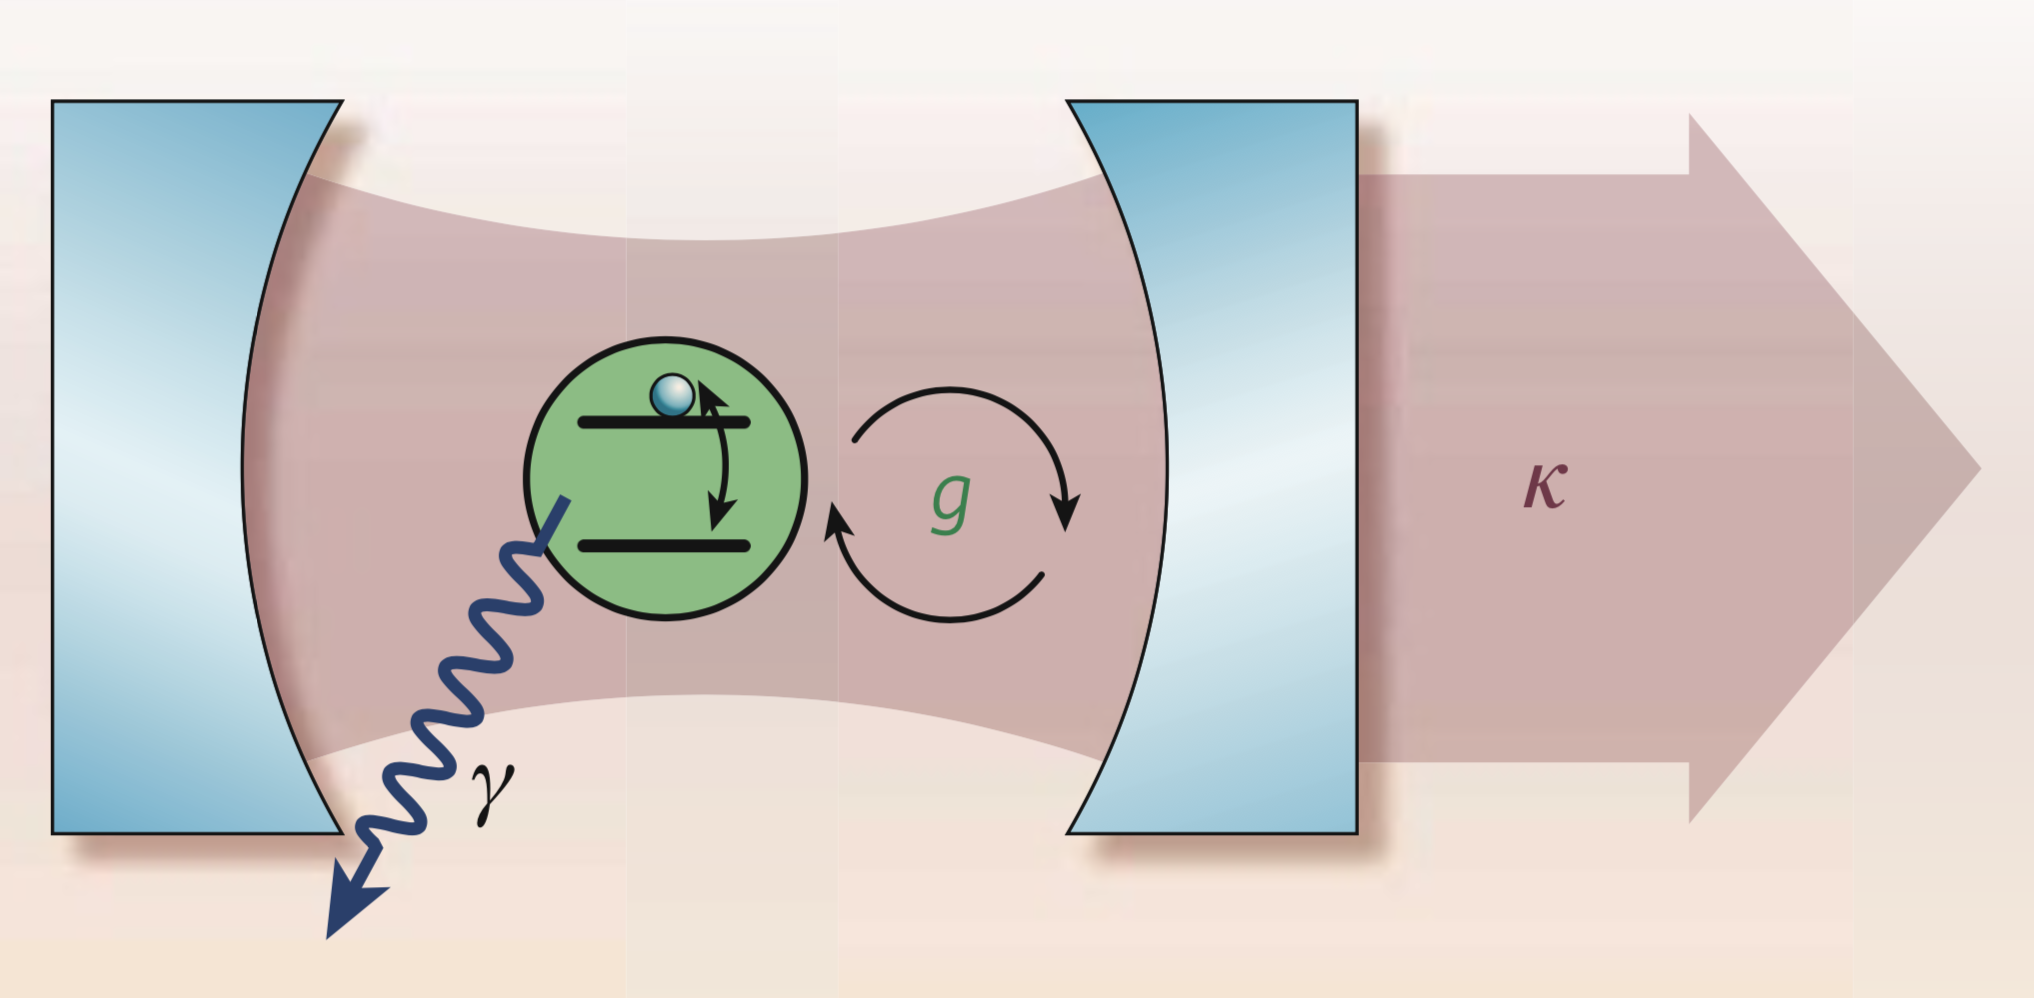
\includegraphics[width=80mm]{fig1.eps}
  \end{center}
  \caption{共振器の量子電磁気学}
\end{figure}

もしこの結合レート$g$が十分に大きければ、励起された原子が自然放出した光子が共振器中を往復し、再び吸収する現象が起こるようになる。これは通常の自然放出とは異なり、コヒーレントな振動現象であって可逆的である。これを真空Rabi振動と呼び、$g$が十分に大きな領域を強結合領域と呼ぶ。真空Rabi振動が観測されるとき光の量子性があらわになり、単一光子レベルでの非線形効果が観測できるようになる。真空Rabi振動は量子情報が原子と光の間で何回も交換されることを意味し、このとき基底状態と励起状態で量子ビットが重ね合わさった状態をとる。

付録Aに示したように、gには上限が存在する。ただし多くの場合、この系で上限近くのgを達成することはとても難しい。そのために次節で説明するような人工原子系で同様の働きをする系が考えだされた。

\section{電気回路上の量子電磁気学 (circuit QED)}
原子を用いた共振器QEDでは大きな結合レートを実現できないため、量子的な電磁気現象を観測するために、散逸の小さな人工的な二準位系とFabry-Perot型共振器の組み合わせが用いられる。その1つのセットアップを模式的に図2に示す。
\begin{figure}[htb]
    \begin{center}
   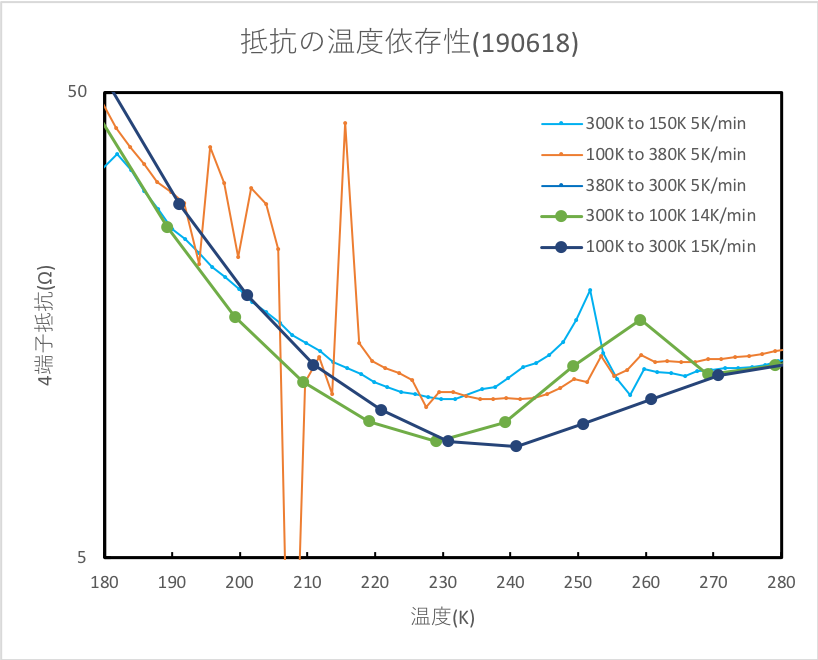
\includegraphics[width=120mm]{fig2.eps}
  \end{center}
  \caption{電気回路上の量子電磁気学}
\end{figure}

入射したマイクロ波(3-30GHz)は超伝導体でできたFabry-Perot型共振器に閉じ込められ定在波をつくる。このとき最大でQ値は$10^6$(光子がロスなく1000回程度往復)となる。定在波の腹付近に人工原子を配置することで、電場が人工原子と相互作用する。

人工原子は図3に等価回路を示すようなJosephson接合からなる。Josephson接合の等価回路のインダクタンス$L_J$は関係$I=I_c sin\psi$と$V=\frac{\hbar}{2e}\frac{\partial \psi}{\partial t}$ から 
\begin{eqnarray}
L_J = \frac{2e}{\hbar} \frac{1}{I_c cos \psi}
\end{eqnarray}
で与えられる。このインダクタンスはJosephson電流$I=I_c sin\psi$に依存するため、等価回路は非線形回路である。したがって$L_J$として量子化をほどこした回路と異なり、エネルギー準位は等間隔とならない。しかし温度をmK領域まで下げると、基底とその上の準位だけに着目した議論が可能である。この準位が人工原子として働く。
\begin{figure}[htb]
    \begin{center}
   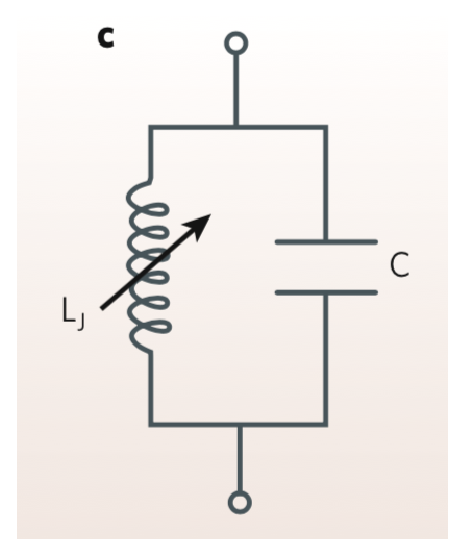
\includegraphics[width=50mm]{fig3.eps}
  \end{center}
  \caption{Josephson接合の等価回路}
\end{figure}

この人工原子が真空Rabi振動状態にある時に、マイクロ波を入射して透過スペクトルを測定すると真空Rabi振動に由来した2つのピークが現れる。このピークを区別することで量子ビットの読み出しを行える。

人工原子の電気双極子モーメントは典型的な原子の10000倍程度になりうる。またこの系は集積回路技術を用いて高精度に加工できるため、空間的に電磁波を閉じ込めることも比較的容易である。さらに、原子を冷却し共振器内にトラップする必要がない。

\appendix
\section{結合レートgの上限}
本節では結合レートgの上限に関して考察する。

まず図1に示したようなキャビティの実効的な半径が$r$で表されるときの電場を見積もる。電子の電気双極子モーメントは原子の特徴長さ$L$を用いて$d=eL$と表されているとする。また共振器の長さを波長の1/2とすると、その長さは$\frac{\pi c}{\omega}$で与えられる。電場のエネルギーは、電磁場の真空揺らぎの半分だから$\frac{\hbar \omega}{4}$である。これを電場のエネルギーの表式$\frac{\epsilon_0}{2}E_0^2 V$と等置すると、
\begin{eqnarray}
E_0 = \frac{1}{r} \sqrt{\frac{\hbar \omega^2}{2\pi^2 \epsilon_0 c} }
\end{eqnarray}
が得られる。

結合レート$g$は$\frac{dE_0}{\hbar}$で与えられるので、$d=eL$の関係を用いて上式から、無次元化された結合レートが見積もられる。
\begin{eqnarray}
\frac{g}{\omega} &=& (\frac{L}{r}) \sqrt{\frac{e^2}{2\pi^2 \epsilon_0 \hbar c} }\\
&=& (\frac{L}{r}) \sqrt{\frac{2\alpha}{\pi} }\\
&\sim& 0.068 (\frac{L}{r} )
\end{eqnarray}
ただし$\alpha\sim1/137$を用いた。$r$は$L$より小さくなることがないので、無次元化された結合レート$g/\omega$の上限は0.068である。


\begin{thebibliography}{9}
\bibitem{Schoelkopf} R. J. Schoelkopf and S. M. Girvin, Wiring up quantum systems, Nature 451, 664 (2008)
\end{thebibliography}

\end{document}